\chapter{Background - Power consumption models in service provider networks}
\label{chap:background}
In this chapter, we first describe the power consumption models for geo-diverse data centers and mobile cellular networks. Then, we draw similarities between these two networks to come up with an abstract power consumption model. This generalized power consumption model motivates the formulation of a generalized electricity cost optimization framework in the next chapter. 

\section{Networks of Geo-Diverse Data Centers - enablers of cloud computing} Traditionally, computational resources are procured, deployed and managed. Authors needing to electronically typeset manuscripts would buy a PC with word-processing software. Organizations that need to deploy an Enterprise Resource Planning (ERP) system would buy servers and install the required software on these. This involves upfront expenditure on equipment and software licensing costs as well as recurring expenses resulting from factors such as renewal of software licenses, salaries for staff to smoothly run the software and training to customize and operate the newly acquired software. 

For much of our non-IT needs, such as electricity, water and gas, we are used to the utility model where we don't own the resources. We pay a per-use subscription charge to some organization that owns and manages the resources for us. Due to economies of scale, utilities are economical for the provider and the end user. It was envisioned that computing could also be offered as a utility, to be consumed and sometimes paid for, as needed. This is the vision of cloud computing. Since our computing needs are met somewhere out there, where we don't know how it is all managed and run, we call it the cloud.

Based on the flexibility and sophistication of the service being offered, cloud computing has various service models, as described below: 

\begin{itemize}
\item \textbf{Infrastructure as a Service (IaaS)}: In this model, the consumer gets access to one or more servers hosted and managed by the service provider. The consumer is responsible for installing the Operating System (OS) and any other software according to their requirements. Amongst all cloud computing models, this one offers the greatest flexibility to the end user. The end user can choose which Operating System they want to run. They can deploy their own customized applications on the server. This also means that the great responsibility of server software management lies on the end user. Amazon Web Services (AWS), Microsoft Azure and Google Compute Engine are examples of IaaS.
\item \textbf{Platform as a Service (PaaS)}: In this model, the service provider offers a complete computing platform with a pre-installed Operating System (OS). The computing platform generally also includes other pre-installed software such as a database management system (DBMS) and programming environment. The service consumer can deploy their required applications on the platform as long as it meets the application's software requirements. Microsoft Azure offers PaaS model services. Hosted web servers are another example of PaaS.
\item \textbf{Software as a Service (SaaS)}: A service user often wishes to be least concerned with software installation, configuration and maintenance. The user just wishes to access an application remotely and seamlessly. The cloud computing model for such cases is SaaS. Web-based email services such as GMail are a common example of SaaS.
\end{itemize}

In order to offer cloud computing, cloud operators deploy large facilities called data centers. A data center may have tens of thousands of servers to provide computing as a utility. Cloud operators typically deploy multiple data centers at different geographic locations. Figure~\ref{fig:googledcmap} shows the locations of Google's data centers across the globe (according to www.google.com/about/datacenters/inside/locations/ as of August 10, 2014).

The geographic distribution of data centers is done for two reasons, namely resilience and lowering client latency. In terms of resilience, having multiple diverse sites helps because if one site goes down, another site may take over. Also, multiple remote sites are less likely to be affected simultaneously by a natural disaster. Furthermore, typically an operator has data centers in different continents, thereby ascertaining that no matter where a client may be, there is a data center relatively close by.. 

\begin{figure}
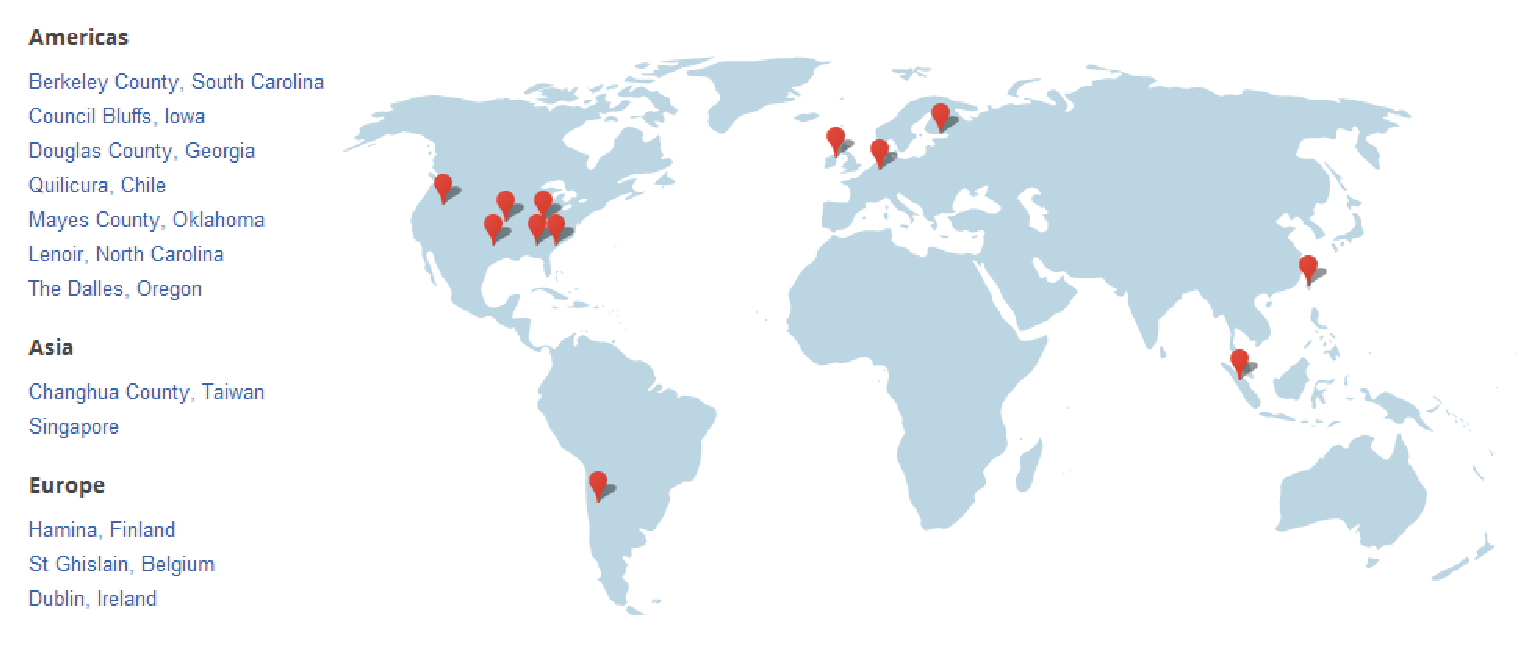
\includegraphics[width=1\textwidth]{pics/googledcmap2.eps}
\label{fig:googledcmap}
\caption{Google Data Center Locations - Source: www.google.com/about/datacenters/inside/locations/}
\end{figure}

\subsection{Structure of a data center} Today's data centers are organized hierarchically~\cite{dcnetworking:vahdat:micro:2010}, as shown in Figure~\ref{fig:dcheir}. A typical data center hosts tens of thousands of servers~\cite{Abts:2012:GTD:2184319.2184335}. The servers are installed in vertical racks. Apart from servers, the racks host other equipment as well. In addition to built-in hard drives in the servers, some dedicated storage nodes are also installed in the racks. A high speed Ethernet switch provides interconnection between the devices installed in the rack and connectivity to the rest of the data center and beyond. Power supply and distribution units for the equipment are also installed in the rack. 

A group of racks, called a pod (or a cluster), are interconnected by means of aggregation switches. An aggregation switch allows servers in different racks to communicate with each other. All the pods within a data center are interconnected by core switches. This allows servers in different pods to communicate with each other. The core switches are interconnected through one or more border routers. These border routers are the avenues for traffic coming in and going out of the data center. 

\begin{figure}
\includegraphics[width=1\textwidth]{pics/dcheir.eps}
\caption{The modern data center's architecture}
\label{fig:dcheir}
\end{figure}

All of the equipment is quite tightly packed in a data center. The equipment generates a lot of heat and to prevent thermal damage to it, cooling must be provided. This is generally done by air-cooling, i.e., heat is transported away from the equipment by circulating cool air around it.

\subsection{Interconnection of data centers} Servers in a data center must often communicate with servers in other data centers. Therefore, each of these data centers is inter-connected by means of high-speed inter data center network links. These links serve to carry various types of traffic, some of which are given below:
\begin{itemize}
\item \textbf{Consistency traffic:} An operator often maintains replicas of some of the servers in their data centers. These replicas are maintained for achieving one or both of the following three objectives: high throughput, resilience and low-latency to clients. Multiple replicas that handle client requests simultaneously can help to increase the effective throughput, i.e., the number of requests handled per second. Sometimes a secondary replica does not actively handle client requests until the primary server fails. When such an event occurs, the secondary replica takes over and offers continued services to the clients. Lastly, by geographically distributing several replicas of a server and routing client requests to the nearest replica, the client latency to the server can be minimized. 

If the content hosted on a server is static, all of its replicas are always automatically consistent, i.e., the user will have the same experience irrespective of the replica that serves its request. However, most applications have data that changes over time. For such applications, whenever content on one server changes, the change must be reflected to all other replicas. For instance, a customer's website may be hosted at two different data centers and whenever a change is made to one copy of the website, the same changes must be reflected at the replica as well. This action requires network traffic between the data centers that host the replicas. 
\item \textbf{Background traffic due to load-balancing:} Some traffic on the inter-data center links may be a result of the effort to achieve load-balancing amongst the data centers. As an example, consider a web-based email service provider that has partitioned user inboxes over the data centers. One objective of this partitioning may be that roughly the same amount of storage space is used at each data center. Since user inbox sizes are dynamic with different growth/shrink rates\footnote{User inbox size grows when new emails are received and shrinks when emails are deleted. Furthermore, the inbox may grow and shrink at different rates, depending on factors such as number of mailing lists that a user subscribes}, the partitioning of users amongst data centers must be dynamic as well. The operator must periodically determine a new user partitioning that results in roughly equal storage space being consumed at each data center. In order to achieve this balanced storage size, some users' inboxes must be moved from one data center to another, over the inter-data center links.
\item \textbf{Background traffic due to distributed computing:} Handling client requests in a distributed fashion requires network traffic overhead due to different servers communicating user requests, intermediate results and final responses. For instance, a web search provider may distributed the web's index over multiple data centers. When a search query is being processed, the request must be sent to all data centers over the inter-data center links and the responses from the data centers, received over these links,  must be aggregated.
\end{itemize}

\subsection{Handling of client requests} 
%front-end server based load balancing and request routing mechanisms such as IP Anycast
We observed in chapter~\ref{chap:intro} that electricity cost depends not only on how much workload is handled, but also where it is handled. Thus, in order to develop a model for electricity cost in a geo-diverse data center, we need to first understand how workload from all over the globe is distributed amongst the data centers. In this section, we will use as an example a client request for viewing a web page hosted by a geo-diverse data center operator. 

To access a web resource, the user types a uniform resource locator (URL) in the web browser's address bar. The URL typically contains the Fully Qualified Domain Name (FQDN), such as www.google.com, corresponding to the web server that hosts the requested resource\footnote{It is also possible to specify the IP address of the web server directly in the URL.}. Since a single server would hardly be sufficient to handle all traffic for a popular web site, several servers are actually mapped to the same FQDN. However, the web browser must connect to exactly one of these servers to fetch a particular web resource. Figure~\ref{fig:dcloadbalance} briefly describes how this web server's IP address is picked.  

\begin{figure}
\centering
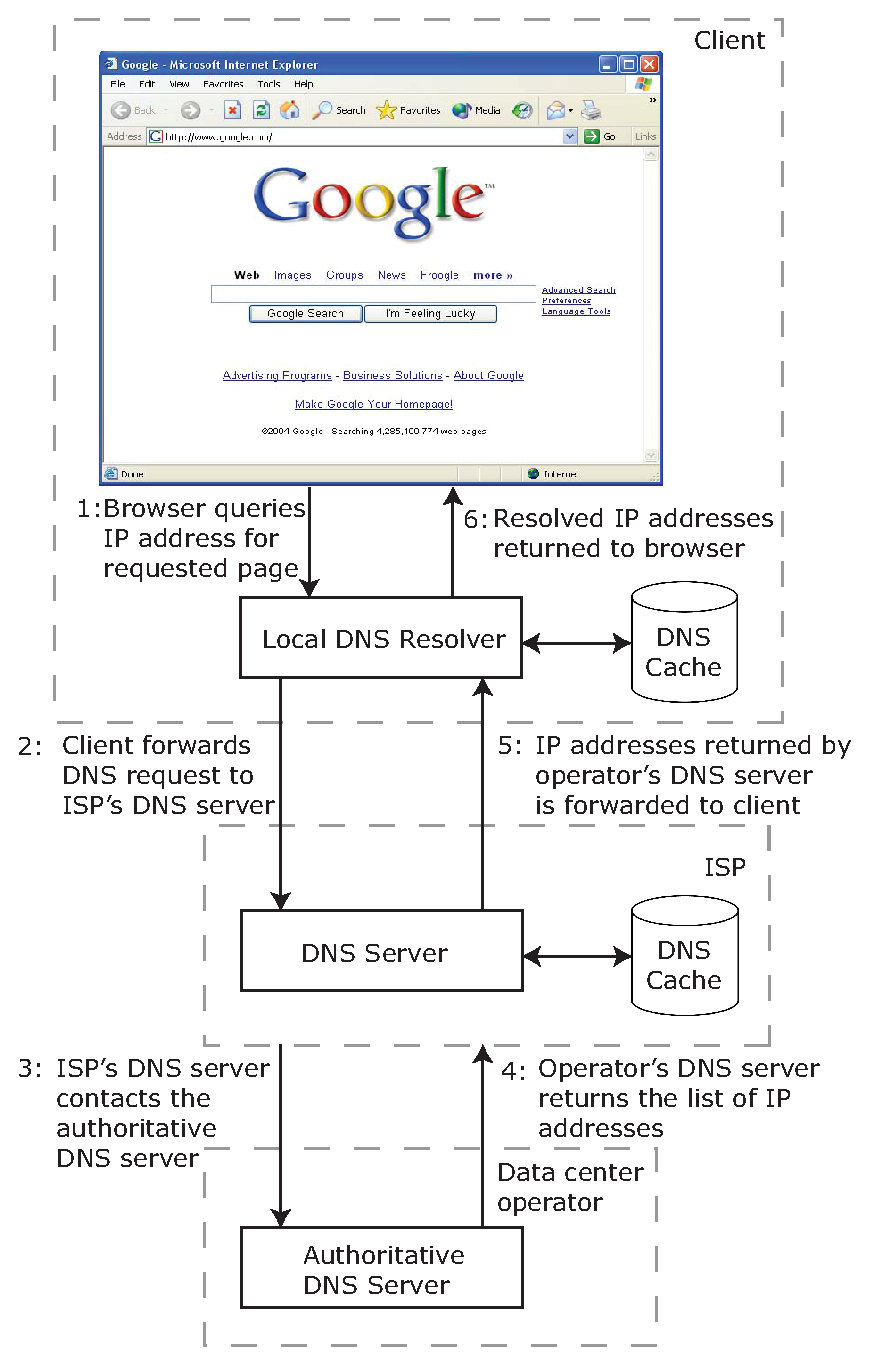
\includegraphics[width=0.5\textwidth]{pics/dcloadbalance.eps}
\caption{Resolving the IP address for a server hosted in a data center}
\label{fig:dcloadbalance}
\end{figure}

The process to view the web page starts with what is known as DNS resolution, which is briefly described here. For details on DNS resolution process, see~\cite{rfc1034,rfc1035}. When the user directs the web browser to fetch a web page by typing a URL in the address bar, the browser invokes the local Domain Name System (DNS) resolver on the client machine which attempts to determine the IP address corresponding to the DNS name of the remote host specified in the URL. The local DNS resolver communicates with the DNS server for the client's ISP\footnote{Some people configure other DNS servers, such as Google's Open DNS Servers on their machines. In such cases, the local DNS resolver would communicate with those other DNS servers.}. The DNS query eventually reaches the authoritative server for the remote host's domain. In our example, this would be operated by the data center operator. The DNS server for the data center operator resolves the DNS name by returning a list of IP addresses corresponding to the servers that are associated with the DNS name specified by the client. When the client receives the DNS response containing list of IP addresses, it picks one of the IP addresses to fetch the web page. For simplicity, many web browsers always pick the first IP address in the list. If the web browser is unable to connect to that IP address, it tries the second one on the list and so on. For consecutive responses to DNS queries for the same FQDN, DNS servers often rotate the list of IP addresses in each response so that if the client always picks the first IP address on the list, the servers are likely to receive equal workload.

Notice in Figure~\ref{fig:dcloadbalance} that caches are available at various DNS resolvers in order to improve the latency of DNS resolution. These caches will keep the list of IP addresses corresponding to recently queried DNS names until the timeout specified by the authoritative DNS server occurs.

The data center operator has a large pool of IP addresses (IP address space) for their layer 3 devices. This IP address space is segmented over the geo-distributed data centers. The IP address picked by the client from amongst the list received from the operator's DNS server belongs to one of these data centers. The client must now send its Hyper Text Transfer Protocol (HTTP)~\cite{rfc1945} request to the server corresponding to the chosen IP address. To this end, the client establishes a Transport Control Protocol (TCP) connection with the server using the selected IP address. An HTTP request is sent over this TCP connection and a response is received. During this communication, packets from the client leave the client's network interface and are routed by the ISPs towards the data center where the required web server is hosted. These packets enter the data center at the border router which forwards these packets to the server with the destination IP address. En-route, these packets traverse the core, aggregation and top of rack switches. The HTTP response packets are forwarded from the web server back to the border router which routes it back to the client machine. Hence, the requested web page is displayed in the client's web browser.

\subsection{Data center power consumption model} 
%Describe the power consumption model from prior work and derive a more simplified yet equivalent model
The electric load within a data center may be categorized into (i) IT load and (ii) non-IT load. The IT load includes servers, network equipment and network storage. The non-IT load includes power supplies, un-interruptible power supplies (UPS), air-conditioning and lighting. 

Fan et. al. used the results of a measurement study to show that the total power consumption in a data center can be well-modeled as an affine function of the average CPU utilization~\cite{Fan:power:ICSA:2007}. As more and more client traffic arrives at servers in a data center, the average CPU utilization increases. Therefore, data center power consumption can also be represented as an affine function of workload. The total power consumption for an operator is the sum of the power consumption over all data centers. 

\section{Cellular Networks} %Just as data centers enable applications that we rely on every day, cellular networks are an important enabler of another pervasive service: telephony.
Mobile telephone systems have enabled not only untethered access to traditional telephony services but also new types of services. We make phone calls, send text messages and can even connect to the Internet using our mobile phones. Just as Internet connectivity services are provided by ISPs and Internet applications are powered by data center operators, mobile phone services are provided by mobile network operators (MNOs).  

Over the years, mobile networks have been deployed based on different technologies. First generation cellular networks (1G) were based on Advanced Mobile Phone System (AMPS). AMPS networks were deployed starting in 1978. The AMPS system also evolved into Digital-AMPS (D-AMPS) networks. Two technologies were part of the second generation (2G) cellular networks, namely Global System for Mobile communication (GSM) and Code Division Multiple Access (CDMA). Anticipating the increased demand for mobile access to data services such as Internet access, vendors introduced General Packet Radio Service (GPRS) as an add-on to GSM networks. GPRS offers data rates between 56 kbps and 114 kbps. A GSM network with GPRS is sometimes referred to as 2.5G. GPRS bit rates are insufficient for many high bandwidth applications such as video calls, video streaming and video conferencing. To enable such services, broadband mobile services were introduced in third generation (3G) networks networks such as High Speed Downlink Packet Access (HSDPA) and Universal Mobile Telephone System (UMTS). The increasing trends in the use of high-bandwidth applications in mobile networks has spawned the fourth generation (4G) cellular networks such as Mobile WiMAX and Long Term Evolution (LTE). In this thesis, we consider only GSM cellular networks.

\subsection{Structure of a cellular network} %A really basic introduction to cellular networks covering: concept of cells, mobile stations (MSs), Base Transceiver Stations (BTSs) and Base Station Controllers (BSCs)
Mobile phone networks are also referred to as cellular networks because the area covered by the operator is logically divided into several small areas called cells. A cell in an urban setting (a macrocell) is typically upto a few hundred meters in radius, whereas in suburban or rural settings, the cell radius may be as large as a few kilometers. A \textit{cell site}, typically situated in the middle of a cell, enables subscribers in that cell to connect to the mobile network. A cell site, often referred to as a Base Transceiver Station (BTS)\footnote{A single cell site sometimes hosts multiple BTSs, for instance, when multiple network operators share a single site} or simply a base station, hosts a number of transceivers (TRXs), radio antennas, power amplifiers and other allied equipment. 

A cell is typically divided into three sectors, resembling 120 degree pie-slices, each covered by different directional antennae. Each sector may have multiple TRXs. A typical cell configuration is one with six TRXs in each cell, referred to as a 6+6+6 cell. 

GSM uses a combination of frequency division multiple access (FDMA) and time division multiple access (TDMA). Each sector is assigned multiple frequency channels. Each frequency is also time-shared between users. Each GSM frame has a duration of 4.6 ms, which is divided into 8 time slots of 0.577 ms each. The transmission within a time slot for a given frequency in termed as a burst. The recurrence of a particular burst across all GSM frames is termed as a physical channel. In other words, there are 8 physical channels per frequency. A few of the physical channels in each sector are reserved for control signaling purposes and the rest can be used for user traffic such as voice calls. Since the number of physical channels represents traffic capacity, and the number of physical channels is proportional to the number of TRXs in a sector, the number of TRXs represents a cell's traffic capacity.

A government regulator such as Pakistan Telecommunication Authority (PTA) allocates a frequency band to each of the operators providing cellular service in the host country. This band The allocation is such that each operator gets a different frequency band. The operator distributes their allocated band to cells in their network. The channels allocated to an operator are much fewer than the number of cells in the network. Therefore, a given channel must be reused in an operator's network. Frequency reuse is done in such a way that any two cells that share the same frequency channel are sufficiently far apart so that the radio signal from any one of the cells does not noticeably interfere with that in the other. In fact, each cell is typically divided into three sectors (resembling 120 degree pie-slices), therefore, the frequency allocation is done on a per-sector basis. Nonetheless, for a high-level view, the set of frequencies allotted to all sectors in a cell can be considered as allotted to the cell itself. Each TRX at a cell site operates at a distinct frequency\footnote{Given two communicating parties at fixed locations, if the transmitted signal power is kept constant, the received radio signal strength would differ depending on the frequency used. Also, this frequency selective behavior of the radio communication medium keeps changing with time, i.e., if frequency A receives better propagation compared to frequency B at time $t_1$, the same will not necessarily be true at time $t_1+\epsilon$. This means that we can't statically pick the best frequencies to use for a particular cell by considering, for instance, the type of terrain. In order to make decent communication conditions available to all callers, on average, GSM networks also use frequency hopping, whereby the frequency allocation to cells are changed periodically.}. 

Frequency assignment and frequency hopping are examples of activities that require coordination. For systematic coordination of radio resources, Base Station Controllers (BSCs) are deployed in the network. The operator's coverage area is geographically split into zones, each of which is controlled by a single BSC. The BTSs communicate with the BSC via backhauls such as E-1 links or microwave. Since a BSC only controls a subset of BTSs, it can only perform local coordination. However, there is a need for global coordination in radio resource allocation. For instance, cells near the boundary of adjacent zones covered by two different BSC must not be assigned the same frequency channels to avoid interference. Therefore, in order to ensure global coordination in radio resource allocation and control, the BSCs are also interconnected using backhaul links.

A mobile station (MS) often receives radio signals from multiple BTSs nearby. The MS picks the BTS from which it receives the strongest signal as its serving BTS. A MS will do all communication such as call reception and placement through the serving BTS. When a subscriber moves around in the operator's coverage area, the signal from the serving BTS might weaken. In such an event, the MS requests the network to allow it to change the serving BTS to the one from which it currently receives the strongest signal. This call handoff is coordinated by a Base Station Controller (BSC). 

Another key component of a GSM network is the Mobile Switching Center (MSC) that is responsible for call routing both within the GSM network and beyond (to a landline phone, for instance). Since the focus of our thesis is power consumption in the network and 50\%~\cite{Louhi:2007:BTSPower:INTELEC} - 80\%~\cite{Oh:Comm:2011} of a cellular network's electricity consumption is due to the BTSs, we will not dwell on the MSC and other components of the cellular network any more than necessary.

\subsection{Call placement} %How a call is handled by a BTS (at a very abstract level, i.e., how is the serving BTS chosen). Role of the BSC in cell association and call hand-off
To place a voice call, when a user enters the phone number digits on the MS and presses the send button, the MS requests the BTS to acquire a channel to communicate with the MSC. Once this channel is successfully acquired, the MSC authenticates the MS, sets up encryption so that the call data is secure. The MS then send the dialed digits to the MSC. The MSC instructs the BSC and MS to switch from signaling mode to voice mode and attempts to route the call to the called numbers. A downlink channel is assigned so that the ringing tone and called party voice can be heard on the calling MS. If there is an error in call establishment, an error message is heard on the calling MS over the same channel. In short, two channels are required to support a voice call in the sector where the call originates.

A sector with $n$ TRXs has $8n$ physical channels. It appears that the sector should be able to support $4n$ calls because each call requires two physical channels. However, the actual maximum number of simultaneous calls is different from this number for two reasons: 
\begin{itemize}
\item Some channels are reserved for control purposes, the exact number of such channels varies from operator to operator.
\item GSM supports two different types of codecs, namely the full-rate codec and the half-rate codec. The full-rate codec corresponds to a caller using a burst in every GSM frame during a call, whereas the half-rate codec corresponds to a caller using a burst in every alternate GSM frame. By default, the full-rate codec is used for every call. However, when traffic congestion rises above an operator-configured threshold, the network attempts to admit every new call using a half-rate codec, if the corresponding MS supports it. If the traffic rises further and crosses a second threshold as configured by the operator, the network also re-assigns current calls to use a half-rate codec depending on the corresponding MS support. This enables a BTS to support more than $8n$ simultaneous calls during times of congestion.
\end{itemize}
 

\subsection{BTS power consumption model} %Describe the power consumption model from prior work
BTSs account for most of the power consumed in a cellular network. Louhi~\cite{Louhi:2007:BTSPower:INTELEC} claimed that BTSs contribute 50\% of overall network power consumption, whereas Oh et. al~\cite{Oh:Comm:2011} put this number at 80\%. For this reason, most of the prior work related to power consumption in cellular networks focuses on BTSs. 

Lorincz et. al. performed a measurement study of BTS power consumption under real-traffic conditions. They concluded that the BTS power consumption may be approximated as an affine function of call traffic~\cite{Lorincz:BTS-Measure:Sensors:2012}. Thus, as traffic varies during a given day, instantaneous power consumption would follow a similar curve as the traffic. 

\section{A comparison of data center and cellular networks} %Geo-diverse data centers and cellular networks are similar in the sense that both are built out of network resources to handle workload which results in electricity consumption. 
\label{sec:chap2:comparison}
\begin{table}
\begin{center}
\begin{tabular}{|c|c|c|}
\hline \ & \textbf{Geo-diverse data centers} & \textbf{GSM cellular networks} \\
\hline \textbf{Traffic Characteristics} & Diurnal patterns & Diurnal patterns \\
\hline \textbf{Network capacity} & Dimensioned according & Dimensioned according \\
\ & to peak workload & to peak workload \\
\hline \textbf{Energy proportionality} & No & No \\
\hline \textbf{Power consumption} & Affine function of workload & Affine function of workload \\
\hline \textbf{Geo-diversity} in & Yes & No \\
\textbf{electricity prices} & \ & \ \\
\hline \textbf{Geo-flexibility in} & \ & \ \\
\textbf{resource selected for} & High & Low \\
\textbf{workload handling} & \ & \ \\
\hline
\end{tabular}
\caption{A comparison of data center and cellular networks}
\label{tab:contrast}
\end{center}
\end{table}

From our discussion of geo-diverse data centers and cellular networks, we note that these networks have several similarities and some subtle differences apropos their power consumption. Keeping their similarities and differences in mind, abstractions can be identified to generically represent these networks. These similarities and differences are summarized in Table~\ref{tab:contrast}. Both of these networks are a collection of resources that handle workload. The resources are data centers and BTSs in case of geo-diverse data centers and cellular networks, respectively. The workload is clients' computing requests such as web page views in case of data centers, whereas it is voice calls in case of cellular networks. The workload in both types of networks exhibits diurnal patterns~\cite{10.1109/MC.2007.443,Peng:2011:TPS:2030613.2030628}. The network in both cases is provisioned according to peak workload demand. Since the network resources are not energy proportional, this means that in low-workload regimes, the network is heavily over-provisioned. Thus, both of these networks are energy inefficient. The power consumption for both networks is an affine function of the workload. 

At any given time, if $x_i$ is the utilization of resource $i$, the power consumption for resource $i$ may be given as:

\begin{align}
P^i = P_{min} + x_i (P_{max} - P_{min})
\end{align}

where $P_{min}$ and $P_{max}$ are the power consumption of a network resource under no-load and full-load respectively. Assuming that the network has a total of $m$ resources, then the network's total instantaneous power consumption may be given as:

\begin{align}
\sum_{i=1}^m \{ P_{min} + x_i (P_{max} - P_{min}) \}
\label{eq:abdcpaper}
\end{align}

Despite the similarity in the power consumption model for both networks, there are some differences as well. One such difference is that the workload in case of geo-diverse data centers may be handled at any of the data centers (assuming that all content is completely replicated on all data centers). However, a voice call may only be served through one of a few candidate BTSs that are near the caller. A result of different geo-flexibility of workload is that in a geo-diverse data center scenario, the candidate serving resources exhibit diversity in electricity prices, because data centers, being far apart, are likely to be under different tariffs. Meanwhile, nearby BTSs are unlikely to be under different tariffs. 

\section{Discussion}
In this chapter, we have seen that there are certain similarities between geo-diverse data centers and cellular networks apropos their power consumption. We have used these similarities to identify abstractions for a general model of power consumption in these networks. Using these abstractions, we identified a generic power consumption model applicable to both geo-diverse data centers and cellular networks. In the next chapter, we will use this model to formulate a generic electricity cost minimization framework.